% Drawing 142/06-9 -- folder 142, batch 06, archive page 109 (PDF page 110).
% Transcription: Sphère centrale, au crayon et à l'encre : sur l'équateur le point $Q_1$ près de $-1$, le cercle autour de $1$ avec $s^+_1$, $s^-_1$, $a^{++}_1$, $a^{+-}_1$ ; chemins $b^+_1$, $b^-_1$ vers les cercles des pôles ($R^-_\infty$, $a^-_\infty$, $R^+_\infty$, $a^+_\infty$) ; inscriptions $d^+_1 (c^+_1)^{-1}$, $(a^-_1 a^+_1)^{-1}$, $d^-_1 (c^-_1)^{-1}$ ; un axe traverse la sphère, une flèche de rotation à côté.
% Kind: sphere with equatorial band, small circles and paths. Method 2 (schematic redraw from the facsimile). Status: partial.
% Notes: Upside-down half of p. 109, redrawn upright. Pencil outline; the pole circles (top: R_infty^-, a_infty^+-; bottom: R_infty^+, a_infty^+-); the inked closed band along the equator through Q_1 (near -1) and round the circle of 1 with s_1^+-, a_1^{++}, a_1^{+-}; dashed paths b_1^+ and b_1^- from Q_1 to the pole circles; the inscriptions d_1^+(c_1^+)^{-1}, (a_1^- a_1^+)^{-1}, d_1^-(c_1^-)^{-1}; the axis through the sphere and the rotation arrow beside it. Which inscription is attached to which stroke is a reading.
% Coordinates: 1 unit = 1 mm = 1/100 of the crop width (bbox in page fractions: [0.204, 0.444, 0.524, 0.642]).
% Redrawn by Claude (claude-opus-5-5), issue #73, 2026-11-07; not checked by a human; not compiled (no TeX in the session).
% Rights: reproduces part of the work -- behind RENDER_TRANSCRIPTS, never published by itself.
\documentclass[tikz,border=3pt]{standalone}
\usepackage{amsmath,amssymb}
\usetikzlibrary{patterns,arrows.meta}
\tikzset{pencil/.style={black!45}, struck/.style={black!35}, mark/.style={circle,draw,inner sep=1.3pt}, pt/.style={circle,fill,inner sep=0.9pt}, opt/.style={circle,draw,fill=white,inner sep=1.1pt}}
\begin{document}
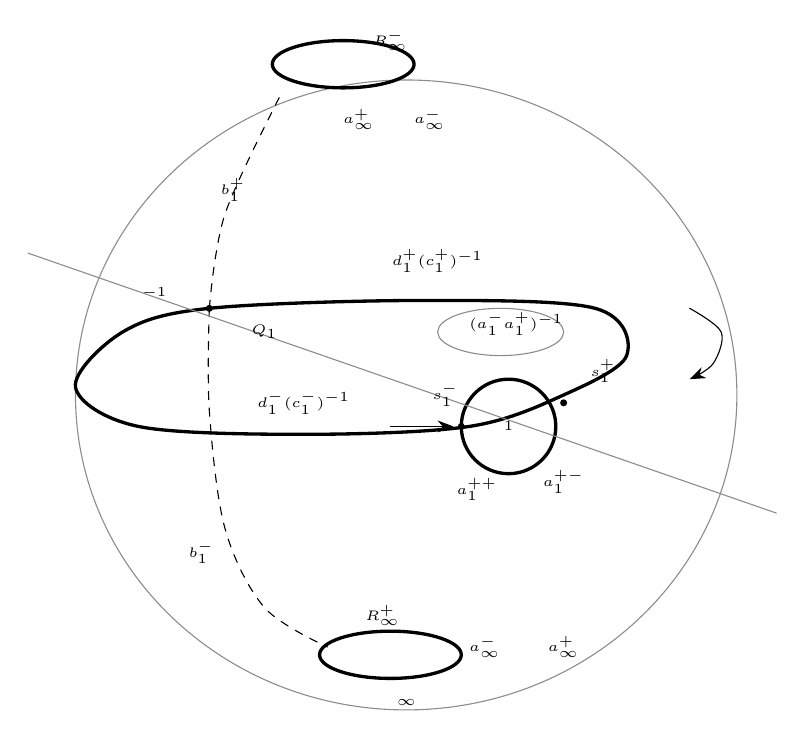
\begin{tikzpicture}[x=1mm,y=1mm,line cap=round,line join=round,font=\scriptsize]
\draw[pencil] (48,-48) ellipse[x radius=42, y radius=40];
\draw[very thick] (40,-6) ellipse[x radius=9, y radius=3];
\draw[very thick] (46,-81) ellipse[x radius=9, y radius=3];
\draw[very thick] plot[smooth cycle, tension=0.55] coordinates {(23,-37) (50,-36) (72,-37) (76,-43) (68,-48) (56,-52) (35,-53) (14,-52) (6,-47) (12,-40)};
\node[pt] at (23,-37) {};
\draw[very thick] (61,-52) circle[radius=6];
\node[pt] at (55,-52) {};
\node[pt] at (68,-49) {};
\draw[-{Stealth[length=2mm]}] (46,-52) -- (54,-52);
\draw[pencil] (60,-40) ellipse[x radius=8, y radius=3];
\draw[dashed] plot[smooth, tension=0.55] coordinates {(23,-37) (25,-25) (32,-10)};
\draw[dashed] plot[smooth, tension=0.55] coordinates {(23,-37) (23,-50) (25,-65) (30,-75) (38,-80)};
\draw[pencil] (0,-30) -- (95,-63);
\draw[-{Stealth[length=2mm]}] plot[smooth, tension=0.55] coordinates {(84,-37) (88,-40) (87,-44) (84,-46)};
\node[inner sep=1pt] at (46,-3) {\tiny $R_\infty^{-}$};
\node[inner sep=1pt] at (42,-13) {\tiny $a_\infty^{+}$};
\node[inner sep=1pt] at (51,-13) {\tiny $a_\infty^{-}$};
\node[inner sep=1pt] at (45,-76) {\tiny $R_\infty^{+}$};
\node[inner sep=1pt] at (58,-80) {\tiny $a_\infty^{-}$};
\node[inner sep=1pt] at (68,-80) {\tiny $a_\infty^{+}$};
\node[inner sep=1pt] at (48,-87) {\tiny $\infty$};
\node[inner sep=1pt] at (26,-22) {\tiny $b_1^{+}$};
\node[inner sep=1pt] at (30,-40) {\tiny $Q_1$};
\node[inner sep=1pt] at (16,-35) {\tiny $-1$};
\node[inner sep=1pt] at (52,-31) {\tiny $d_1^{+}(c_1^{+})^{-1}$};
\node[inner sep=1pt] at (62,-39) {\tiny $(a_1^{-}a_1^{+})^{-1}$};
\node[inner sep=1pt] at (35,-49) {\tiny $d_1^{-}(c_1^{-})^{-1}$};
\node[inner sep=1pt] at (53,-48) {\tiny $s_1^{-}$};
\node[inner sep=1pt] at (73,-45) {\tiny $s_1^{+}$};
\node[inner sep=1pt] at (61,-52) {\tiny $1$};
\node[inner sep=1pt] at (57,-60) {\tiny $a_1^{++}$};
\node[inner sep=1pt] at (68,-59) {\tiny $a_1^{+-}$};
\node[inner sep=1pt] at (22,-68) {\tiny $b_1^{-}$};
\end{tikzpicture}
\end{document}
